% =============================================================================
%  Diplomado en Data Science Aplicada con Python para la Toma de Decisiones
%  Clase 36: RAG multimodal --- por qué tu PDF rompe el RAG simple
%  Arca Continental Ecuador | UDLA
% =============================================================================
\documentclass[aspectratio=169, 11pt]{beamer}

\usepackage[T1]{fontenc}
\usepackage[utf8]{inputenc}
\usepackage[spanish,es-noshorthands]{babel}
\usepackage{FiraSans}
\usepackage{FiraMono}
\renewcommand{\familydefault}{\sfdefault}
\usepackage{graphicx}
\usepackage{tikz}
\usetikzlibrary{arrows.meta, positioning, shapes.geometric, shapes.misc,
  calc, fit, decorations.pathreplacing, backgrounds, matrix, chains}
\usepackage{fontawesome5}
\usepackage{minted}
\usepackage{tcolorbox}
\tcbuselibrary{minted, skins, breakable}
\usepackage{booktabs}
\usepackage{multicol}
\usepackage{hyperref}
\usepackage{calc}
\usepackage{amsmath}

\definecolor{arcaRed}{HTML}{C82B40}
\definecolor{arcaDark}{HTML}{6B1525}
\definecolor{arcaGray}{HTML}{F5F5F5}
\definecolor{arcaLightGray}{HTML}{EBEBEB}
\definecolor{textDark}{HTML}{2D2D2D}
\definecolor{textMuted}{HTML}{6B7280}
\definecolor{codeGreen}{HTML}{16A34A}
\definecolor{codeBlue}{HTML}{2563EB}
\definecolor{codeOrange}{HTML}{EA580C}
\definecolor{codePurple}{HTML}{7C3AED}

\usetheme{default}
\usecolortheme{default}
\setbeamertemplate{navigation symbols}{}
\setbeamertemplate{footline}{}
\setbeamertemplate{headline}{}
\setbeamercolor{normal text}{fg=textDark}
\setbeamercolor{frametitle}{fg=arcaRed, bg=white}
\setbeamercolor{title}{fg=white}
\setbeamercolor{subtitle}{fg=white!85}
\setbeamercolor{author}{fg=white!80}
\setbeamercolor{date}{fg=white!70}
\setbeamercolor{item}{fg=arcaRed}
\setbeamercolor{subitem}{fg=arcaDark}
\setbeamerfont{frametitle}{size=\Large, series=\bfseries}
\setbeamerfont{title}{size=\huge, series=\bfseries}
\setbeamerfont{subtitle}{size=\large}
\setbeamertemplate{itemize item}{\scriptsize\raise1.5pt\hbox{\color{arcaRed}$\blacktriangleright$}}
\setbeamertemplate{itemize subitem}{\scriptsize\raise1pt\hbox{\color{arcaDark}$\bullet$}}
\setbeamertemplate{enumerate items}[default]
\setbeamercolor{enumerate item}{fg=arcaRed}

\setbeamertemplate{headline}{%
  \begin{tikzpicture}[remember picture, overlay]
    \fill[arcaDark] (current page.north west) rectangle
      ([yshift=-0.7cm]current page.north east);
    \node[anchor=west, inner sep=0pt] at
      ([xshift=0.6cm, yshift=-0.35cm]current page.north west)
      {
\includegraphics[height=0.45cm]{../logo_udla_white.png}};
    \node[anchor=east, inner sep=0pt] at
      ([xshift=-0.6cm, yshift=-0.35cm]current page.north east)
      {
\includegraphics[height=0.45cm]{../ArcaContinental_white.png}};
  \end{tikzpicture}%
  \vspace{0.7cm}%
}

\setbeamertemplate{footline}{%
  \begin{tikzpicture}[remember picture, overlay]
    \node[anchor=south east, font=\scriptsize\bfseries\color{arcaRed}] at
      ([xshift=-0.5cm, yshift=0.15cm]current page.south east)
      {\insertframenumber};
  \end{tikzpicture}%
  \vspace{0.3cm}%
}

\setbeamertemplate{frametitle}{%
  \vspace{0.25cm}%
  \usebeamerfont{frametitle}\usebeamercolor[fg]{frametitle}\insertframetitle%
  \par\vspace{2pt}%
  \begin{tikzpicture}
    \fill[arcaRed] (0,0) rectangle (3cm, 1.5pt);
    \fill[arcaLightGray] (3cm,0) rectangle (\textwidth, 0.5pt);
  \end{tikzpicture}%
  \vspace{0.1cm}%
}

\newtcblisting{pyblock}[1][]{%
  listing engine=minted, minted language=python, minted style=friendly,
  minted options={fontsize=\small, linenos=false, breaklines=true, python3=true},
  colback=arcaGray, colframe=arcaRed, left=4pt, right=4pt, top=4pt, bottom=4pt,
  boxrule=0pt, leftrule=3pt, arc=2pt, listing only, #1}

\newcommand{\sectionframe}[2]{%
  \begingroup
  \setbeamertemplate{headline}{}%
  \setbeamertemplate{footline}{}%
  \begin{frame}[plain, noframenumbering]
    \begin{tikzpicture}[remember picture, overlay]
      \fill[arcaRed] (current page.south west) rectangle (current page.north east);
      \node[anchor=center, text=white, font=\Huge\bfseries, text width=12cm,
            align=center] at ([yshift=0.5cm]current page.center) {#1};
      \node[anchor=center, text=white!80, font=\large, text width=10cm,
            align=center] at ([yshift=-0.8cm]current page.center) {#2};
    \end{tikzpicture}
  \end{frame}
  \endgroup
}

\tikzset{
  arrowR/.style={-{Stealth[length=2.5mm]}, arcaRed, thick},
  arrowD/.style={-{Stealth[length=2.5mm]}, arcaDark, thick},
  arrowG/.style={-{Stealth[length=2.5mm]}, color=textMuted, thick, dashed},
  boxA/.style={rectangle, rounded corners=4pt, draw=arcaDark, fill=arcaGray,
               align=center, font=\footnotesize, inner sep=4pt, minimum height=0.9cm},
  boxRed/.style={rectangle, rounded corners=4pt, draw=arcaDark, fill=arcaRed,
                 text=white, align=center, font=\bfseries\footnotesize,
                 inner sep=5pt, minimum height=0.9cm},
  boxBlue/.style={rectangle, rounded corners=4pt, draw=arcaDark, fill=codeBlue,
                  text=white, align=center, font=\bfseries\footnotesize,
                  inner sep=5pt, minimum height=0.9cm},
  boxGreen/.style={rectangle, rounded corners=4pt, draw=arcaDark, fill=codeGreen,
                   text=white, align=center, font=\bfseries\footnotesize,
                   inner sep=5pt, minimum height=0.9cm},
  boxOrange/.style={rectangle, rounded corners=4pt, draw=arcaDark, fill=codeOrange,
                    text=white, align=center, font=\bfseries\footnotesize,
                    inner sep=5pt, minimum height=0.9cm},
  boxPurple/.style={rectangle, rounded corners=4pt, draw=arcaDark, fill=codePurple,
                    text=white, align=center, font=\bfseries\footnotesize,
                    inner sep=5pt, minimum height=0.9cm},
}

\title{Diplomado en Data Science Aplicada\\con Python para la Toma de Decisiones}
\subtitle{Clase 36: RAG multimodal --- por qué tu PDF rompe el RAG simple}
\author{Carlos Enrique Mosquera Trujillo}
\date{9 de Junio, 2026}

\begin{document}

% =====================================================================
%  F1 — PORTADA
% =====================================================================
{
\setbeamertemplate{headline}{}
\setbeamertemplate{footline}{}
\begin{frame}[plain, noframenumbering]
  \begin{tikzpicture}[remember picture, overlay]
    \fill[arcaDark] (current page.south west) rectangle (current page.north east);
    \fill[arcaRed] ([yshift=-3.5cm]current page.north west) rectangle
      ([yshift=-4.2cm]current page.north east);
    \node[anchor=west, inner sep=0pt] at
      ([xshift=1cm, yshift=-1.5cm]current page.north west)
      {
\includegraphics[height=1cm]{../logo_udla_white.png}};
    \node[anchor=east, inner sep=0pt] at
      ([xshift=-1cm, yshift=-1.5cm]current page.north east)
      {
\includegraphics[height=1cm]{../ArcaContinental_white.png}};
  \end{tikzpicture}
  \vspace{2.5cm}
  \begin{center}
    {\usebeamerfont{title}\usebeamercolor[fg]{title}\inserttitle\par}
    \vspace{0.4cm}
    {\usebeamerfont{subtitle}\usebeamercolor[fg]{subtitle}\insertsubtitle\par}
    \vspace{0.6cm}
    {\usebeamerfont{author}\usebeamercolor[fg]{author}\insertauthor\par}
    \vspace{0.15cm}
    {\usebeamerfont{date}\usebeamercolor[fg]{date}\insertdate\par}
  \end{center}
\end{frame}
}

% =====================================================================
%  F2 — Dónde quedamos en clase 35
% =====================================================================
\begin{frame}[shrink]{Dónde quedamos en la clase 35}
  \vspace{6pt}
  \begin{center}
  \begin{tikzpicture}[node distance=0.4cm and 0.4cm, font=\footnotesize]
    \node[boxA, minimum width=2.6cm] (q) {Pregunta};
    \node[boxBlue, right=of q] (e) {Embed};
    \node[boxOrange, right=of e] (db) {Buscar\\en NumPy};
    \node[boxGreen, right=of db] (top) {Top-K\\chunks};
    \node[boxRed, right=of top] (llm) {LLM\\(Llama 3.1-8B)};
    \node[fill=arcaDark, text=white, rounded corners=4pt, font=\bfseries\footnotesize,
          right=of llm, inner sep=5pt] (ans) {Respuesta\\+ cita};
    \draw[arrowR] (q) -- (e); \draw[arrowR] (e) -- (db);
    \draw[arrowR] (db) -- (top); \draw[arrowR] (top) -- (llm);
    \draw[arrowR] (llm) -- (ans);
  \end{tikzpicture}
  \end{center}
  \vspace{14pt}
  \begin{tcolorbox}[colback=arcaGray, colframe=arcaRed, leftrule=3pt,
    boxrule=0pt, sharp corners, left=8pt, right=8pt, top=6pt, bottom=6pt]
    {\footnotesize\color{arcaDark}
    Armamos el \textbf{chatbot Arca de Ética y Cumplimiento}: indexamos un PDF
    de 8 páginas (el código de ética público), corrimos PyPDF, chunkeamos,
    embebimos con \texttt{mpnet} y buscamos por coseno. Funcionó. Citaba
    el documento y rechazaba los 3 ataques de injection.}
  \end{tcolorbox}
  \vspace{6pt}
  \begin{tcolorbox}[colback=arcaRed!8, colframe=arcaRed, leftrule=3pt,
    boxrule=0pt, sharp corners, left=8pt, right=8pt, top=4pt, bottom=4pt]
    {\footnotesize\color{arcaDark}\bfseries
    Funcionó porque el PDF era texto plano, sin figuras complicadas.
    \emph{Hoy le tiramos un PDF real.}}
  \end{tcolorbox}
\end{frame}

% =====================================================================
%  F3 — La pregunta del día
% =====================================================================
\begin{frame}[shrink]{La pregunta del día}
  \vspace{12pt}
  \begin{center}
  \begin{tcolorbox}[colback=arcaDark, colframe=arcaDark, sharp corners,
    boxrule=0pt, left=14pt, right=14pt, top=12pt, bottom=12pt, width=0.92\textwidth]
    {\normalsize\color{white}\bfseries
    En clase 35 armamos un chatbot Arca que cita el Código de Ética. Hoy queremos
    uno que lea el \textbf{Reporte Anual Integrado 2025} de Arca Continental:
    189 páginas, 415 figuras, gráficos de sostenibilidad, tablas financieras.
    ¿Por qué el RAG simple se rompe aquí, qué le ponemos para que funcione, y
    cuánto código real escribimos --- vs. cuánto le pedimos a una librería
    profesional?\par}
  \end{tcolorbox}
  \end{center}
  \vspace{14pt}
  \begin{tcolorbox}[colback=arcaRed!8, colframe=arcaRed, leftrule=3pt,
    boxrule=0pt, sharp corners, left=8pt, right=8pt, top=4pt, bottom=4pt]
    {\footnotesize\color{arcaDark}\bfseries
    Acompaña los 6 bloques. La respondemos al final, frame 49.}
  \end{tcolorbox}
\end{frame}

% =============================================================================
%  BLOQUE 0 — RAG: qué, para qué, cómo combate la alucinación
% =============================================================================
\sectionframe{Bloque 0}{RAG: qué es,\\para qué sirve,\\y cómo le tapa la boca al modelo que inventa}

% F5 — ¿Qué es RAG?
\begin{frame}[shrink]{¿Qué es RAG, en una frase?}
  \vspace{12pt}
  \begin{center}
  \begin{tcolorbox}[colback=arcaGray, colframe=arcaRed, sharp corners,
    leftrule=4pt, boxrule=0pt, left=14pt, right=14pt, top=10pt, bottom=10pt,
    width=0.88\textwidth]
    {\normalsize\color{arcaDark}\bfseries
    \emph{Retrieval-Augmented Generation}: antes de responder, el modelo
    \textbf{recupera} los documentos relevantes y \textbf{los pega} en su
    propio contexto.\par}
  \end{tcolorbox}
  \end{center}
  \vspace{14pt}
  \begin{center}
  \begin{tikzpicture}[font=\footnotesize, node distance=0.4cm and 0.5cm]
    \node[boxA, minimum width=2.4cm] (q) {Pregunta\\del usuario};
    \node[boxBlue, right=of q] (r) {Recupero\\docs relevantes};
    \node[fill=arcaDark, text=white, rounded corners=4pt, right=of r,
          minimum width=2.6cm, minimum height=0.9cm, align=center,
          font=\bfseries\footnotesize] (llm) {LLM\\con contexto};
    \node[boxGreen, right=of llm] (a) {Respuesta\\$+$ cita};
    \draw[arrowR] (q) -- (r); \draw[arrowR] (r) -- (llm); \draw[arrowR] (llm) -- (a);
  \end{tikzpicture}
  \end{center}
  \vspace{12pt}
  \begin{tcolorbox}[colback=arcaRed!8, colframe=arcaRed, leftrule=3pt,
    boxrule=0pt, sharp corners, left=8pt, right=8pt, top=4pt, bottom=4pt]
    {\footnotesize\color{arcaDark}\bfseries
    Idea grande: \emph{primero buscar, después hablar.}}
  \end{tcolorbox}
\end{frame}

% F6 — ¿Para qué sirve?
\begin{frame}[shrink]{¿Para qué sirve RAG --- 3 casos típicos en Arca}
  \vspace{10pt}
  \begin{center}
  \begin{tikzpicture}[node distance=0.5cm and 0.5cm, font=\footnotesize]
    \node[fill=codeBlue!15, draw=codeBlue, rounded corners=4pt,
          minimum width=4.0cm, minimum height=2.0cm, align=center,
          font=\bfseries\footnotesize] (a)
          {\faBook\\\textbf{Consultar políticas}\\\tiny ``¿cómo reporto algo anónimo?''\\\tiny respuesta cita el manual};
    \node[fill=codeOrange!15, draw=codeOrange, rounded corners=4pt,
          minimum width=4.0cm, minimum height=2.0cm, align=center,
          font=\bfseries\footnotesize, right=of a] (b)
          {\faChartLine\\\textbf{Analizar reportes}\\\tiny ``¿qué metas de\\\tiny sostenibilidad para 2030?''};
    \node[fill=codeGreen!15, draw=codeGreen, rounded corners=4pt,
          minimum width=4.0cm, minimum height=2.0cm, align=center,
          font=\bfseries\footnotesize, right=of b] (c)
          {\faHeadset\\\textbf{Atender clientes}\\\tiny FAQ + tickets pasados\\\tiny sin alucinar};
  \end{tikzpicture}
  \end{center}
  \vspace{14pt}
  \begin{tcolorbox}[colback=arcaGray, colframe=arcaRed, leftrule=3pt,
    boxrule=0pt, sharp corners, left=8pt, right=8pt, top=6pt, bottom=6pt]
    {\footnotesize\color{arcaDark}
    El factor común: \textbf{el modelo solo, sin contexto, inventa.}
    Le damos los documentos \textbf{a la hora de responder} y el problema desaparece.}
  \end{tcolorbox}
\end{frame}

% F7 — Cómo combate la alucinación
\begin{frame}[shrink]{Cómo combate la alucinación}
  \vspace{8pt}
  \begin{columns}[t]
    \begin{column}{0.47\textwidth}
      \begin{center}
      \begin{tcolorbox}[colback=arcaRed!10, colframe=arcaRed,
        sharp corners, boxrule=0pt, leftrule=3pt, left=8pt, right=8pt,
        top=4pt, bottom=4pt, title={\scriptsize\color{white}\bfseries SIN RAG},
        coltitle=white, colbacktitle=arcaRed, fonttitle=\scriptsize]
      \begin{tikzpicture}[font=\scriptsize, node distance=0.3cm]
        \node[boxA] (q) {pregunta};
        \node[fill=arcaDark, text=white, rounded corners=4pt, right=of q,
              minimum width=1.6cm, minimum height=0.7cm, font=\bfseries\scriptsize] (l) {LLM};
        \node[fill=arcaRed, text=white, rounded corners=4pt, right=of l,
              minimum width=2.0cm, minimum height=0.7cm, font=\bfseries\scriptsize] (a)
              {respuesta\\\emph{\tiny inventada}};
        \draw[arrowR] (q) -- (l); \draw[arrowR] (l) -- (a);
      \end{tikzpicture}
      \end{tcolorbox}
      \end{center}
      \vspace{4pt}
      {\footnotesize\color{arcaDark}
      El modelo genera ``el código de ética dice…''\par
      sin haber visto el código de ética.\par
      Puede acertar de casualidad. O inventar.}
    \end{column}
    \begin{column}{0.47\textwidth}
      \begin{center}
      \begin{tcolorbox}[colback=codeGreen!10, colframe=codeGreen,
        sharp corners, boxrule=0pt, leftrule=3pt, left=8pt, right=8pt,
        top=4pt, bottom=4pt, title={\scriptsize\color{white}\bfseries CON RAG},
        coltitle=white, colbacktitle=codeGreen, fonttitle=\scriptsize]
      \begin{tikzpicture}[font=\scriptsize, node distance=0.3cm]
        \node[boxA] (q) {pregunta};
        \node[boxBlue, right=of q] (r) {top-K\\docs};
        \node[fill=arcaDark, text=white, rounded corners=4pt, right=of r,
              minimum width=1.4cm, minimum height=0.7cm, font=\bfseries\scriptsize] (l) {LLM};
        \node[fill=codeGreen, text=white, rounded corners=4pt, right=of l,
              minimum width=1.8cm, minimum height=0.7cm, font=\bfseries\scriptsize] (a)
              {respuesta\\\emph{\tiny + cita}};
        \draw[arrowR] (q) -- (r); \draw[arrowR] (r) -- (l); \draw[arrowR] (l) -- (a);
      \end{tikzpicture}
      \end{tcolorbox}
      \end{center}
      \vspace{4pt}
      {\footnotesize\color{arcaDark}
      El modelo lee \textbf{el chunk literal}\par
      antes de contestar.\par
      Si la respuesta no está en el contexto,\par
      la instrucción es \emph{``decí no aparece''}.}
    \end{column}
  \end{columns}
  \vspace{8pt}
  \begin{tcolorbox}[colback=arcaRed!8, colframe=arcaRed, leftrule=3pt,
    boxrule=0pt, sharp corners, left=8pt, right=8pt, top=3pt, bottom=3pt]
    {\footnotesize\color{arcaDark}\bfseries
    No es magia: el modelo \emph{sigue pudiendo} inventar. Pero la
    tasa cae fuerte cuando le pones el documento delante.}
  \end{tcolorbox}
\end{frame}

% F8 — Cierre B0
\begin{frame}[shrink]{\faIndustry\ ¿Qué me llevo? --- Bloque 0}
  \vspace{8pt}
  \begin{itemize}\setlength{\itemsep}{6pt}
    \footnotesize
    \item \textbf{RAG = recuperar antes de generar.}
    Esa es la idea grande.
    \item Sirve cuando el modelo \emph{solo} no tiene esa info confiable
    (políticas internas, reportes propios, FAQ).
    \item \textbf{Es la defensa más fuerte contra alucinación}, junto con
    \texttt{temperature=0} y un buen system prompt.
  \end{itemize}
  \vspace{14pt}
  \begin{tcolorbox}[colback=arcaRed!8, colframe=arcaRed, leftrule=3pt,
    boxrule=0pt, sharp corners, left=8pt, right=8pt, top=4pt, bottom=4pt]
    {\footnotesize\color{arcaDark}\bfseries
    \emph{RAG = recuperar antes de generar. Eso es lo que mata la alucinación.}
    \faArrowRight\;Bloque 1: el RAG simple que ya armaste en clase 35.}
  \end{tcolorbox}
\end{frame}

% =============================================================================
%  BLOQUE 1 — RAG simple (recap clase 35)
% =============================================================================
\sectionframe{Bloque 1}{RAG simple\\(esto ya lo armaste en clase 35)}

% F10 — Pipeline 3 pasos (rehecho con dos filas claras)
\begin{frame}[shrink]{El pipeline de clase 35 --- 3 pasos}
  \vspace{10pt}
  \begin{center}
  \begin{tikzpicture}[font=\footnotesize, node distance=0.45cm and 0.45cm]
    %% Fila 1: INDEXAR (offline)
    \node[font=\bfseries\footnotesize\color{codeBlue}, anchor=west]
         at (-0.5, 1.0) {1.\;INDEXAR \tiny\itshape\color{textMuted}(se hace una vez)};
    \node[boxA, minimum width=1.6cm] (pdf) at (0, 0) {PDF};
    \node[boxA, minimum width=1.8cm, right=of pdf] (ch) {chunkear};
    \node[boxA, minimum width=2.0cm, right=of ch] (em) {embed (mpnet)};
    \node[boxBlue, minimum width=2.0cm, right=of em] (st) {vector store};
    \draw[arrowR] (pdf) -- (ch); \draw[arrowR] (ch) -- (em); \draw[arrowR] (em) -- (st);

    %% Fila 2: RECUPERAR + GENERAR (online)
    \node[font=\bfseries\footnotesize\color{codeOrange}, anchor=west]
         at (-0.5, -1.5) {2.\;RECUPERAR \;+\; 3.\;GENERAR \tiny\itshape\color{textMuted}(cada vez que alguien pregunta)};
    \node[boxA, minimum width=1.8cm] (q) at (0, -2.5) {pregunta};
    \node[boxA, minimum width=1.6cm, right=of q] (qe) {embed};
    \node[boxA, minimum width=1.6cm, right=of qe] (top) {top-K};
    \node[fill=arcaDark, text=white, rounded corners=4pt, right=of top,
          minimum width=1.6cm, minimum height=0.9cm, align=center,
          font=\bfseries\footnotesize] (llm) {LLM};
    \node[boxGreen, minimum width=2.0cm, right=of llm] (ans) {respuesta};
    \draw[arrowR] (q) -- (qe); \draw[arrowR] (qe) -- (top);
    \draw[arrowR] (top) -- (llm); \draw[arrowR] (llm) -- (ans);
    %% Conexion vector store -> top-K (rama dashed)
    \draw[arrowR, dashed, color=textMuted] (st.south) to[bend left=10] (top.north);
  \end{tikzpicture}
  \end{center}
  \vspace{14pt}
  \begin{tcolorbox}[colback=arcaGray, colframe=arcaRed, leftrule=3pt,
    boxrule=0pt, sharp corners, left=8pt, right=8pt, top=4pt, bottom=4pt]
    {\footnotesize\color{arcaDark}
    Tres pasos. \textbf{Indexar} se hace una vez. \textbf{Recuperar} y
    \textbf{generar} se hacen \emph{cada vez} que alguien pregunta.}
  \end{tcolorbox}
\end{frame}

% F11 — El chatbot Ética que funcionó
\begin{frame}[fragile, shrink]{El chatbot Ética que sí funcionó}
  \vspace{4pt}
  \begin{pyblock}
texto  = "\n".join(p.extract_text() for p in PdfReader("etica.pdf").pages)
chunks = [c for c in texto.split("\n\n") if len(c) > 80]

embs = embedder.encode(chunks, normalize_embeddings=True)
def rag(q, k=3):
    qe = embedder.encode([q], normalize_embeddings=True)[0]
    top = np.argsort(-(embs @ qe))[:k]
    return llm(SYSTEM, "CONTEXTO:\n" + "\n---\n".join(chunks[i] for i in top) +
                       f"\n\nPREGUNTA: {q}")
  \end{pyblock}
  \vspace{6pt}
  \begin{tcolorbox}[colback=arcaRed!8, colframe=arcaRed, leftrule=3pt,
    boxrule=0pt, sharp corners, left=8pt, right=8pt, top=3pt, bottom=3pt]
    {\footnotesize\color{arcaDark}\bfseries
    \emph{¿Por qué funcionó?} El PDF de Ética era \textbf{texto plano} y los chunks
    `\texttt{split("\textbackslash n\textbackslash n")}' tenían sentido.
    Si el PDF tiene figuras, columnas, tablas\ldots\ esa última línea se cae.}
  \end{tcolorbox}
\end{frame}

% F12 — Cierre B1
\begin{frame}[shrink]{\faIndustry\ ¿Qué me llevo? --- Bloque 1}
  \vspace{8pt}
  \begin{itemize}\setlength{\itemsep}{6pt}
    \footnotesize
    \item El \textbf{pipeline 3 pasos} (indexar / recuperar / generar) sigue siendo el mismo.
    \item Lo que cambia hoy: \textbf{el primer paso}. Cómo entra el PDF a tu sistema.
    \item Todo lo demás (embedder, vector store, LLM, retrieval) lo dejamos tal cual.
  \end{itemize}
  \vspace{12pt}
  \begin{tcolorbox}[colback=arcaRed!8, colframe=arcaRed, leftrule=3pt,
    boxrule=0pt, sharp corners, left=8pt, right=8pt, top=4pt, bottom=4pt]
    {\footnotesize\color{arcaDark}\bfseries
    \emph{Tres pasos. Texto plano, esto ya lo haces.}
    \faArrowRight\;Bloque 2: ahora le tiramos un PDF real y vemos cómo se rompe.}
  \end{tcolorbox}
\end{frame}

% =============================================================================
%  BLOQUE 2 — Cuando el PDF rompe el RAG simple
% =============================================================================
\sectionframe{Bloque 2}{Cuando el PDF\\rompe el RAG simple}

% F14 — Anatomía de un PDF
\begin{frame}[shrink]{Un PDF no es un \texttt{.txt}}
  \vspace{8pt}
  \begin{columns}[t]
    \begin{column}{0.58\textwidth}
      \begin{center}
      \begin{tikzpicture}[font=\scriptsize]
        % Capas apiladas
        \draw[fill=arcaGray, draw=arcaDark, thick]
          (0,0) rectangle (5, 0.8) node[pos=0.5] {\bfseries Layout (columnas, posiciones)};
        \draw[fill=codePurple!20, draw=arcaDark, thick]
          (0,0.8) rectangle (5, 1.6) node[pos=0.5] {\bfseries Figuras (PNG / vectoriales)};
        \draw[fill=codeOrange!20, draw=arcaDark, thick]
          (0,1.6) rectangle (5, 2.4) node[pos=0.5] {\bfseries Tablas};
        \draw[fill=codeBlue!20, draw=arcaDark, thick]
          (0,2.4) rectangle (5, 3.2) node[pos=0.5] {\bfseries Texto principal};
        \draw[fill=codeGreen!20, draw=arcaDark, thick]
          (0,3.2) rectangle (5, 4.0) node[pos=0.5] {\bfseries Encabezados / pie};
        % Flecha lateral
        \draw[arrowR] (5.4, 2.8) -- (6.6, 2.8) node[midway, above, font=\scriptsize] {PyPDF};
        \node[fill=arcaRed, text=white, rounded corners=2pt, right=6.6,
              minimum width=2cm, minimum height=0.7cm, font=\bfseries\footnotesize,
              align=center] at (6.6,2.8) (out) {sólo\\texto};
      \end{tikzpicture}
      \end{center}
    \end{column}
    \begin{column}{0.42\textwidth}
      \begin{tcolorbox}[colback=arcaGray, colframe=arcaRed, leftrule=3pt,
        boxrule=0pt, sharp corners, left=6pt, right=6pt, top=4pt, bottom=4pt]
        {\scriptsize\color{arcaDark}
        Un PDF guarda \textbf{varias capas} encima de la página. PyPDF lee la
        capa de texto y la concatena \emph{como cadena lineal}, perdiendo el
        contexto visual.}
      \end{tcolorbox}
      \vspace{6pt}
      \begin{itemize}\setlength{\itemsep}{2pt}
        \scriptsize
        \item Las \textbf{figuras} no las ve.
        \item Las \textbf{tablas} las aplana en sopa de números.
        \item Las \textbf{columnas} las mezcla.
      \end{itemize}
    \end{column}
  \end{columns}
\end{frame}

% F15 — El reporte Arca real (screenshot)
\begin{frame}[shrink]{El paciente: página 44 del Reporte Arca 2025}
  \vspace{2pt}
  \begin{columns}[c]
    \begin{column}{0.42\textwidth}
      \begin{center}
      \fbox{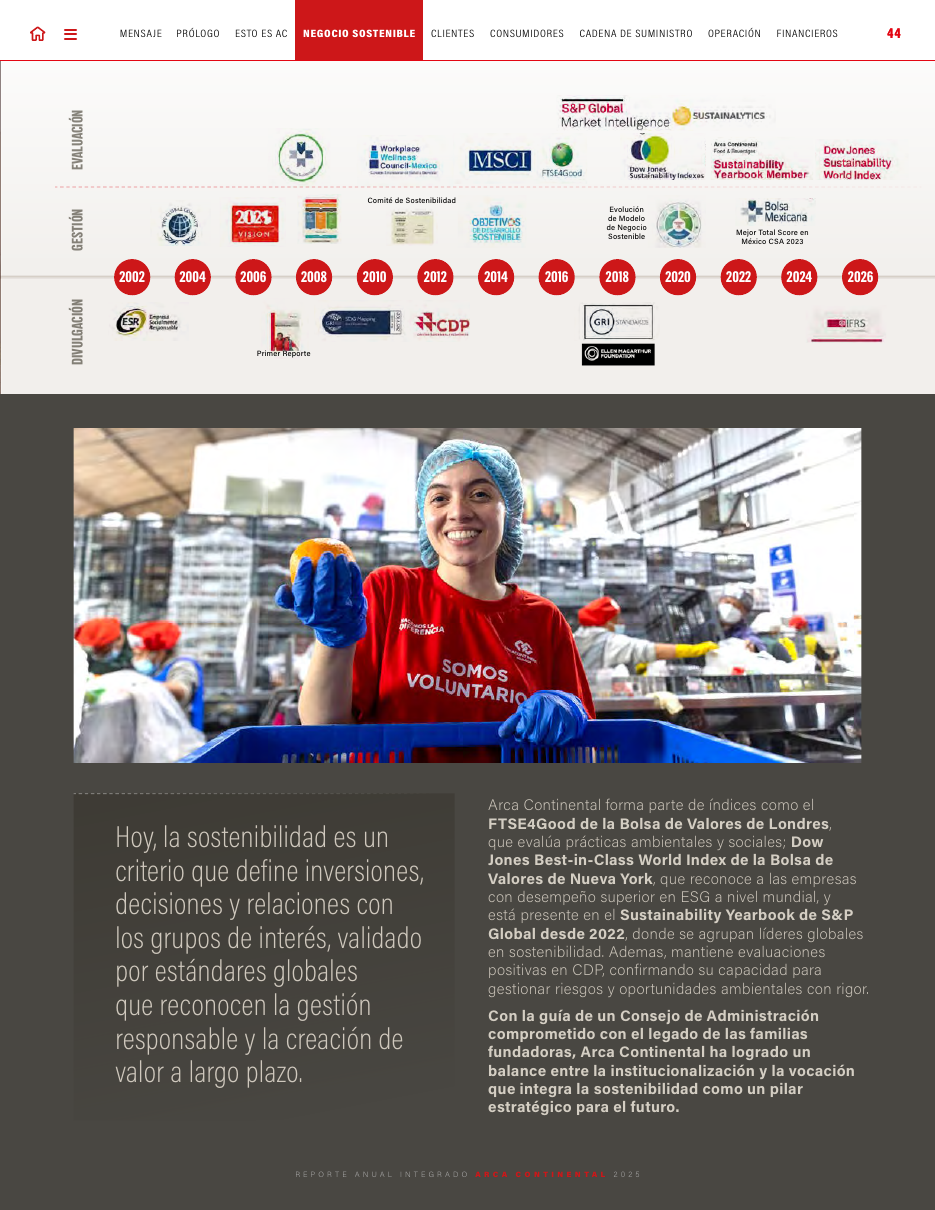
\includegraphics[width=\textwidth]{screenshots/reporte_pag44.png}}
      \end{center}
    \end{column}
    \begin{column}{0.54\textwidth}
      {\scriptsize\color{arcaDark}
      Una página típica de un reporte corporativo real:\par}
      \vspace{4pt}
      \begin{itemize}\setlength{\itemsep}{2pt}
        \scriptsize
        \item Encabezado con \textbf{menú} de secciones.
        \item Una \textbf{barra con 22 logos} de organismos
        (FTSE4Good, S\&P, MSCI\ldots).
        \item Una \textbf{foto} grande de una trabajadora.
        \item \textbf{Tres columnas} de texto.
        \item Un \textbf{recuadro destacado} con el título de la sección.
      \end{itemize}
      \vspace{4pt}
      \begin{tcolorbox}[colback=arcaRed!8, colframe=arcaRed, leftrule=3pt,
        boxrule=0pt, sharp corners, left=5pt, right=5pt, top=3pt, bottom=3pt]
        {\scriptsize\color{arcaDark}\bfseries
        Veámosla primero. Después la pasamos por PyPDF.}
      \end{tcolorbox}
    \end{column}
  \end{columns}
\end{frame}

% F16 — PyPDF crudo sobre esa página
\begin{frame}[fragile, shrink]{Lo que PyPDF saca de esa página (output real)}
  \vspace{2pt}
  \begin{tcolorbox}[colback=arcaGray, colframe=arcaRed, leftrule=3pt,
    boxrule=0pt, sharp corners, left=8pt, right=8pt, top=4pt, bottom=4pt,
    title={\scriptsize\color{white}\bfseries\ttfamily PdfReader("reporte\textunderscore arca.pdf").pages[43].extract\textunderscore text()},
    coltitle=white, colbacktitle=arcaRed, fonttitle=\scriptsize]
    {\scriptsize\color{textDark}\ttfamily
    DIVULGACIÓN GESTIÓN EVALUACIÓN\par
    Comité~~~~de~~~~Sostenibilidad\par
    Evolución~~~~de~~~~Modelo~~~~de~~~~Negocio\par
    S\par
    ostenible\par
    Hoy, la sostenibilidad es un\par
    criterio que define inversiones,\par
    decisiones y relaciones con\par
    los grupos de interés, validado\par
    por estándares globales\par
    Arca Continental forma parte de índices como el\par
    FTSE4Good de la Bolsa de Valores de Londres,\par
    que evalúa prácticas\par
    Dow Jones Best\par
    {\color{arcaRed}\bfseries\textperiodcentered}\par
    in\par
    {\color{arcaRed}\bfseries\textperiodcentered}\par
    Class World Index de la Bolsa de\par}
  \end{tcolorbox}
  \vspace{6pt}
  \begin{tcolorbox}[colback=arcaRed!8, colframe=arcaRed, leftrule=3pt,
    boxrule=0pt, sharp corners, left=8pt, right=8pt, top=3pt, bottom=3pt]
    {\footnotesize\color{arcaDark}\bfseries
    \faExclamationTriangle~``S \textbackslash n ostenible'', ``Dow Jones Best \textbackslash n \textperiodcentered\
    \textbackslash n in \textbackslash n \textperiodcentered\ \textbackslash n Class''. \emph{Las palabras se rompen.}
    Y todo viene en una columna mezclada.}
  \end{tcolorbox}
\end{frame}

% F17 — ¿Y las figuras?
\begin{frame}[shrink]{Y las 22 figuras de esa página\ldots ¿dónde están?}
  \vspace{8pt}
  \begin{center}
  \begin{tikzpicture}[font=\footnotesize, node distance=0.5cm and 0.4cm]
    % PDF con varias capas
    \node[fill=arcaGray, draw=arcaDark, rounded corners=4pt,
          minimum width=2.8cm, minimum height=4.0cm, align=center] (pdf) {};
    \node[font=\bfseries\footnotesize\color{arcaDark}] at ([yshift=1.4cm]pdf) {página 44};
    \node[fill=codeBlue!30, rounded corners=2pt,
          minimum width=2.2cm, minimum height=0.4cm] at ([yshift=0.95cm]pdf.center) {\tiny texto};
    \node[fill=codePurple!30, rounded corners=2pt,
          minimum width=2.2cm, minimum height=0.4cm] at ([yshift=0.45cm]pdf.center) {\tiny 22 logos};
    \node[fill=codeOrange!30, rounded corners=2pt,
          minimum width=2.2cm, minimum height=0.4cm] at ([yshift=-0.05cm]pdf.center) {\tiny foto};
    \node[fill=codeGreen!30, rounded corners=2pt,
          minimum width=2.2cm, minimum height=0.4cm] at ([yshift=-0.55cm]pdf.center) {\tiny 3 columnas};
    \node[fill=arcaRed!30, rounded corners=2pt,
          minimum width=2.2cm, minimum height=0.4cm] at ([yshift=-1.05cm]pdf.center) {\tiny timeline};

    % PyPDF
    \node[fill=arcaDark, text=white, rounded corners=4pt,
          minimum width=2.2cm, minimum height=1cm, font=\bfseries,
          right=2.0cm of pdf] (py) {PyPDF};
    \draw[arrowR] (pdf) -- (py);
    \node[boxA, right=2.0cm of py, minimum width=2.6cm, align=center] (out)
         {sólo el\\\bfseries texto sucio};
    \draw[arrowR] (py) -- (out);

    % Lo que se pierde (debajo)
    \node[font=\scriptsize\itshape\color{arcaRed}, below=1.0cm of py, align=center]
         (lost) {se pierden:\\22 logos $+$ foto $+$ layout\\$=$ \emph{invisibles al RAG}};
    \draw[arrowR, dashed, color=arcaRed] (py.south) -- (lost);
  \end{tikzpicture}
  \end{center}
  \vspace{10pt}
  \begin{tcolorbox}[colback=arcaRed!8, colframe=arcaRed, leftrule=3pt,
    boxrule=0pt, sharp corners, left=8pt, right=8pt, top=3pt, bottom=3pt]
    {\footnotesize\color{arcaDark}\bfseries
    Si alguien te pregunta \emph{``¿en qué índices ESG está Arca?''} y la
    respuesta solo está en los \textbf{logos visuales}\ldots\ tu RAG no lo
    encuentra.}
  \end{tcolorbox}
\end{frame}

% F18 — ¿Y las tablas?
\begin{frame}[shrink]{Y las tablas terminan así\ldots}
  \vspace{6pt}
  \begin{columns}[t]
    \begin{column}{0.45\textwidth}
      \begin{center}
      \begin{tikzpicture}[font=\scriptsize]
        % Tabla visual
        \draw[fill=arcaRed!20, draw=arcaDark] (0,2.4) rectangle (4.6, 3.0);
        \node[font=\bfseries\scriptsize\color{white}] at (2.3,2.7)
              {{\color{arcaDark} código ~~~ equipo ~~~ acción}};
        \foreach \y/\a/\b/\c in
          {1.8/ERR-001/Compresor/Verificar rodamientos.,
           1.2/ERR-002/Llenadora/Limpiar filtro entrada.,
           0.6/ERR-003/Etiquetador/Ajustar rodillo aplicador.}
        {
          \draw[draw=arcaDark!40] (0,\y) rectangle (4.6, \y+0.6);
          \node[anchor=west, font=\scriptsize] at (0.1, \y+0.3) {\a};
          \node[anchor=west, font=\scriptsize] at (1.4, \y+0.3) {\b};
          \node[anchor=west, font=\scriptsize] at (2.8, \y+0.3) {\c};
        }
      \end{tikzpicture}
      \end{center}
      \vspace{4pt}
      {\scriptsize\centering\color{textMuted}\itshape Cómo se ve en el PDF\par}
    \end{column}
    \begin{column}{0.52\textwidth}
      \begin{tcolorbox}[colback=arcaGray, colframe=arcaRed, leftrule=3pt,
        boxrule=0pt, sharp corners, left=6pt, right=6pt, top=4pt, bottom=4pt,
        title={\scriptsize\color{white}\bfseries\ttfamily PyPDF},
        coltitle=white, colbacktitle=arcaRed, fonttitle=\scriptsize]
        {\scriptsize\color{textDark}\ttfamily
        ``código equipo acción ERR-001 Compresor\par
        Verificar rodamientos. ERR-002 Llenadora\par
        Limpiar filtro entrada. ERR-003 Etiquetador\par
        Ajustar rodillo aplicador.''}
      \end{tcolorbox}
      \vspace{4pt}
      {\scriptsize\color{arcaDark}
      Los \textbf{tres campos de cada fila} quedan pegados con el header y con
      las filas siguientes. El RAG ve \emph{una sopa}, no una tabla.}
    \end{column}
  \end{columns}
  \vspace{8pt}
  \begin{tcolorbox}[colback=arcaRed!8, colframe=arcaRed, leftrule=3pt,
    boxrule=0pt, sharp corners, left=8pt, right=8pt, top=3pt, bottom=3pt]
    {\footnotesize\color{arcaDark}\bfseries
    Si preguntas ``¿qué hago con ERR-002?'', el chunk recuperado puede traer
    la acción de ERR-003 mezclada.}
  \end{tcolorbox}
\end{frame}

% F19 — Por qué pasa
\begin{frame}[shrink]{¿Por qué pasa esto?}
  \vspace{8pt}
  \begin{tcolorbox}[colback=arcaGray, colframe=arcaRed, leftrule=3pt,
    boxrule=0pt, sharp corners, left=8pt, right=8pt, top=6pt, bottom=6pt]
    {\footnotesize\color{arcaDark}
    Un PDF está pensado para que un \emph{humano} mire la página y entienda dónde
    está cada cosa. \textbf{No para que una máquina lo lea linealmente.}\par
    \vspace{4pt}
    PyPDF te entrega el texto en \emph{el orden en el que el PDF lo guarda
    internamente} --- que muchas veces es por bloques, columnas o fragmentos
    sueltos sin saber a cuál pertenece cada uno.}
  \end{tcolorbox}
  \vspace{10pt}
  \begin{itemize}\setlength{\itemsep}{4pt}
    \footnotesize
    \item \textbf{Las figuras} son un objeto aparte. PyPDF las salta.
    \item \textbf{Las tablas} no tienen ``modo tabla'' --- son rectangulitos con texto.
    \item \textbf{El layout} (columnas, recuadros, márgenes) PyPDF no lo respeta.
  \end{itemize}
  \vspace{6pt}
  \begin{tcolorbox}[colback=arcaRed!8, colframe=arcaRed, leftrule=3pt,
    boxrule=0pt, sharp corners, left=8pt, right=8pt, top=3pt, bottom=3pt]
    {\footnotesize\color{arcaDark}\bfseries
    Resumen: PyPDF \textbf{no lee mal}. Es que el PDF \emph{no es un .txt} y
    necesitamos más herramientas.}
  \end{tcolorbox}
\end{frame}

% F20 — Cierre B2
\begin{frame}[shrink]{\faIndustry\ ¿Qué me llevo? --- Bloque 2}
  \vspace{6pt}
  \begin{itemize}\setlength{\itemsep}{5pt}
    \footnotesize
    \item Tu \textbf{chatbot de clase 35 SIRVE} cuando el PDF es texto plano (ej.\ el
    código de ética).
    \item Sobre un \textbf{reporte real con figuras, tablas, columnas} --- el
    parser solo de PyPDF no alcanza.
    \item Las \textbf{figuras} se pierden completamente. Las \textbf{tablas} se
    convierten en sopa. El \textbf{layout} se mezcla.
  \end{itemize}
  \vspace{10pt}
  \begin{tcolorbox}[colback=arcaRed!8, colframe=arcaRed, leftrule=3pt,
    boxrule=0pt, sharp corners, left=8pt, right=8pt, top=4pt, bottom=4pt]
    {\footnotesize\color{arcaDark}\bfseries
    \emph{Un PDF real es más complejo de lo que PyPDF puede leer.}
    \faArrowRight\;Bloque 3: para entender lo que el PDF SÍ tiene
    (figuras), necesitamos \emph{modelos multimodales}.}
  \end{tcolorbox}
\end{frame}

% =============================================================================
%  BLOQUE 3 — Modelos multimodales
% =============================================================================
\sectionframe{Bloque 3}{Modelos multimodales\\(el modelo también puede ver)}

% F22 — ¿Qué es multimodal?
\begin{frame}[shrink]{¿Qué quiere decir ``multimodal''?}
  \vspace{8pt}
  \begin{tcolorbox}[colback=arcaGray, colframe=arcaRed, sharp corners,
    boxrule=0pt, leftrule=4pt, left=14pt, right=14pt, top=6pt, bottom=6pt]
    {\footnotesize\color{arcaDark}
    Hasta ahora nuestros modelos recibían \textbf{una sola modalidad}: texto.\par
    Un \emph{modelo multimodal} acepta \textbf{texto + imagen} (o audio, o video)
    \textbf{en la misma llamada}, y la respuesta es texto.}
  \end{tcolorbox}
  \vspace{14pt}
  \begin{center}
  \begin{tikzpicture}[font=\footnotesize, node distance=0.4cm and 0.6cm]
    \node[boxA, minimum width=2.6cm, align=center] (t)
         {\textquotedbl ¿qué\\codigo de error\\veo?\textquotedbl};
    \node[fill=codePurple, text=white, rounded corners=4pt,
          minimum width=2.6cm, minimum height=1.6cm, align=center,
          font=\bfseries\footnotesize, below=0.4cm of t]
          (im) {\faImage\\imagen\\del panel};
    \node[fill=arcaDark, text=white, rounded corners=4pt,
          right=1.6cm of t.east, anchor=west,
          minimum width=2.8cm, minimum height=1.6cm, align=center,
          font=\bfseries\footnotesize, yshift=-0.7cm]
          (m) {modelo\\multimodal\\\tiny(VLM)};
    \node[boxGreen, right=1.0cm of m, minimum width=3.6cm, align=center] (out)
         {\textquotedbl ERR-007:\\presión baja CAB-2\textquotedbl};
    \draw[arrowR] (t.east) to[bend left=10] (m.west);
    \draw[arrowR] (im.east) to[bend right=10] (m.west);
    \draw[arrowR] (m) -- (out);
  \end{tikzpicture}
  \end{center}
\end{frame}

% F23 — Llama 4 Scout
\begin{frame}[shrink]{El modelo que vamos a usar --- Llama 4 Scout 17B}
  \vspace{6pt}
  \begin{center}
  \begin{tabular}{p{3.2cm} p{8.6cm}}
    \toprule
    \scriptsize\textbf{Por qué este} & \scriptsize\textbf{}\\
    \midrule
    \scriptsize\textbf{Mismo proveedor} & \scriptsize Groq, el que ya conocemos de clase 34-35.\\
    \scriptsize\textbf{Cliente idéntico} & \scriptsize El mismo \texttt{client.chat.completions.create()} de la API OpenAI.\\
    \scriptsize\textbf{Free tier} & \scriptsize Suficiente para indexar un reporte completo con cuidado.\\
    \scriptsize\textbf{Acepta base64} & \scriptsize Vos le pasas la imagen como \texttt{data:image/png;base64,\ldots}\\
    \scriptsize\textbf{Reemplazo} & \scriptsize Llama 3.2 Vision \textbf{ya no está} en Groq; Scout es el sucesor.\\
    \bottomrule
  \end{tabular}
  \end{center}
  \vspace{12pt}
  \begin{tcolorbox}[colback=arcaRed!8, colframe=arcaRed, leftrule=3pt,
    boxrule=0pt, sharp corners, left=8pt, right=8pt, top=4pt, bottom=4pt]
    {\footnotesize\color{arcaDark}\bfseries
    Nada de stack nuevo. Los mismos 5 imports. Solo cambia \texttt{model="..."}
    y el formato del mensaje (lista con texto + imagen).}
  \end{tcolorbox}
\end{frame}

% F24 — Anatomía del request
\begin{frame}[fragile, shrink]{Anatomía del request multimodal}
  \begin{pyblock}
import base64
with open("figura.png", "rb") as f:
    b64 = base64.b64encode(f.read()).decode()

r = client.chat.completions.create(
    model="meta-llama/llama-4-scout-17b-16e-instruct",
    messages=[{"role": "user", "content": [
        {"type": "text",      "text": "Describe esta imagen en 2 frases."},
        {"type": "image_url", "image_url": {"url": f"data:image/png;base64,{b64}"}},
    ]}],
    max_tokens=200, temperature=0,
)
print(r.choices[0].message.content)
  \end{pyblock}
  \vspace{4pt}
  \begin{tcolorbox}[colback=arcaGray, colframe=arcaRed, leftrule=3pt,
    boxrule=0pt, sharp corners, left=8pt, right=8pt, top=3pt, bottom=3pt]
    {\footnotesize\color{arcaDark}
    Lo único \emph{nuevo}: \texttt{content} ahora es una \textbf{lista} con
    dos partes (texto $+$ image\textunderscore url) en vez de un \texttt{str}.}
  \end{tcolorbox}
\end{frame}

% F25 — Demo: foto del reporte + pregunta
\begin{frame}[shrink]{Demo en vivo --- una foto del reporte $+$ una pregunta}
  \vspace{2pt}
  \begin{columns}[t]
    \begin{column}{0.36\textwidth}
      \begin{center}
      \fbox{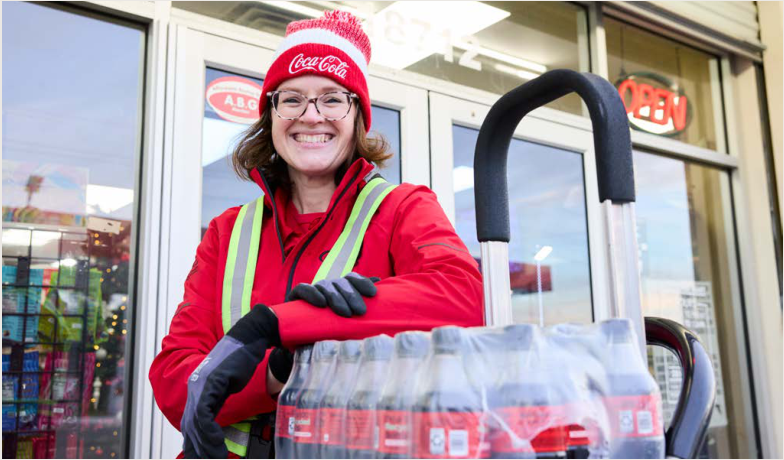
\includegraphics[width=\textwidth]{figs/fig_mujer_cocacola.png}}
      \end{center}
      \vspace{2pt}
      {\scriptsize\itshape\color{textMuted} figura extraída del reporte (pag.\ 52 aprox.)\par}
    \end{column}
    \begin{column}{0.6\textwidth}
      \begin{tcolorbox}[colback=arcaGray, colframe=codeBlue, leftrule=3pt,
        boxrule=0pt, sharp corners, left=6pt, right=6pt, top=4pt, bottom=4pt,
        title={\scriptsize\color{white}\bfseries Prompt},
        coltitle=white, colbacktitle=codeBlue, fonttitle=\scriptsize]
        {\scriptsize\color{textDark}\ttfamily
        ``Describe esta foto en 2 frases. ¿Quién aparece? ¿Qué está haciendo?''}
      \end{tcolorbox}
      \vspace{4pt}
      \begin{tcolorbox}[colback=arcaGray, colframe=codeGreen, leftrule=3pt,
        boxrule=0pt, sharp corners, left=6pt, right=6pt, top=4pt, bottom=4pt,
        title={\scriptsize\color{white}\bfseries Respuesta REAL de Scout},
        coltitle=white, colbacktitle=codeGreen, fonttitle=\scriptsize]
        {\scriptsize\color{textDark}\itshape
        ``En la imagen se ve a una mujer sonriente con un gorro de Coca Cola.
        La mujer está apoyando sus brazos sobre una carga de botellas de Coca Cola
        que transporta en un carrito.''}
      \end{tcolorbox}
      \vspace{6pt}
      \begin{tcolorbox}[colback=arcaRed!8, colframe=arcaRed, leftrule=3pt,
        boxrule=0pt, sharp corners, left=6pt, right=6pt, top=3pt, bottom=3pt]
        {\footnotesize\color{arcaDark}\bfseries
        Reconoce el gorro, la marca, las botellas, el carrito.
        Eso es lo que necesitamos.}
      \end{tcolorbox}
    \end{column}
  \end{columns}
\end{frame}

% F26 — Cierre B3
\begin{frame}[shrink]{\faIndustry\ ¿Qué me llevo? --- Bloque 3}
  \vspace{6pt}
  \begin{itemize}\setlength{\itemsep}{5pt}
    \footnotesize
    \item \textbf{Multimodal} no es ciencia rara. Es ``el modelo también puede ver''.
    \item En Groq: una sola línea cambia. Mismo cliente, mismo patrón.
    \item Lo que recibe el modelo sigue siendo \emph{prompt $+$ contexto}. Solo que
    ahora el contexto puede incluir \emph{una imagen}.
  \end{itemize}
  \vspace{12pt}
  \begin{tcolorbox}[colback=arcaRed!8, colframe=arcaRed, leftrule=3pt,
    boxrule=0pt, sharp corners, left=8pt, right=8pt, top=4pt, bottom=4pt]
    {\footnotesize\color{arcaDark}\bfseries
    \emph{Multimodal $=$ el modelo no solo lee, también ve.}
    \faArrowRight\;Bloque 4: y cuando le pedimos \emph{que describa una imagen
    con palabras}, eso se llama \textbf{captioning}.}
  \end{tcolorbox}
\end{frame}

% =============================================================================
%  BLOQUE 4 — Image captioning
% =============================================================================
\sectionframe{Bloque 4}{Image captioning\\(la imagen se vuelve texto)}

% F28 — ¿Qué es captioning?
\begin{frame}[shrink]{¿Qué es \emph{image captioning}?}
  \vspace{12pt}
  \begin{center}
  \begin{tikzpicture}[font=\footnotesize, node distance=0.4cm and 0.6cm]
    \node[fill=codePurple, text=white, rounded corners=4pt,
          minimum width=2.4cm, minimum height=1.6cm, align=center,
          font=\bfseries\footnotesize] (im) {\faImage\\imagen};
    \node[fill=arcaDark, text=white, rounded corners=4pt, right=of im,
          minimum width=2.4cm, minimum height=1.6cm, align=center,
          font=\bfseries\footnotesize] (m) {VLM\\(Scout)};
    \node[boxA, right=of m, minimum width=4.0cm, align=center]
         (out) {\textquotedbl una mujer con gorro\\ de Coca-Cola, sobre\\botellas en un carrito\textquotedbl};
    \draw[arrowR] (im) -- (m); \draw[arrowR] (m) -- (out);
  \end{tikzpicture}
  \end{center}
  \vspace{14pt}
  \begin{tcolorbox}[colback=arcaGray, colframe=arcaRed, leftrule=3pt,
    boxrule=0pt, sharp corners, left=8pt, right=8pt, top=6pt, bottom=6pt]
    {\footnotesize\color{arcaDark}
    Le pides al VLM una sola cosa: \emph{``descríbeme esta imagen en X frases''}.
    Sale \textbf{texto}. \textbf{Y eso es lo que mete tu RAG al vector store.}}
  \end{tcolorbox}
\end{frame}

% F29 — Para qué sirve en RAG
\begin{frame}[shrink]{Por qué resuelve el problema}
  \vspace{6pt}
  \begin{center}
  \begin{tikzpicture}[font=\footnotesize, node distance=0.45cm]
    \node[fill=codePurple!20, draw=arcaDark, rounded corners=4pt,
          minimum width=2.0cm, minimum height=1.2cm, align=center]
          (i) {\faImage\\figura};
    \node[fill=arcaDark, text=white, rounded corners=4pt, right=of i,
          minimum width=2.0cm, minimum height=1.2cm, align=center,
          font=\bfseries\footnotesize] (s) {Scout\\caption};
    \node[boxA, right=of s, minimum width=2.4cm] (t) {texto};
    \node[boxBlue, right=of t, minimum width=2.0cm] (e) {embed\\mpnet};
    \node[fill=codeGreen, text=white, rounded corners=4pt,
          right=of e, minimum width=1.8cm, minimum height=1.0cm,
          align=center, font=\bfseries\footnotesize] (v) {vector};
    \draw[arrowR] (i) -- (s); \draw[arrowR] (s) -- (t);
    \draw[arrowR] (t) -- (e); \draw[arrowR] (e) -- (v);
  \end{tikzpicture}
  \end{center}
  \vspace{14pt}
  \begin{itemize}\setlength{\itemsep}{5pt}
    \footnotesize
    \item La imagen entra como texto al vector store.
    \item \textbf{Tu RAG de clase 35 SIGUE FUNCIONANDO} sin cambios.
    \item Cuando alguien pregunta ``¿qué muestra el panel de la línea 2?'', el
    chunk recuperado puede ser \emph{el caption de una foto}.
  \end{itemize}
  \vspace{6pt}
  \begin{tcolorbox}[colback=arcaRed!8, colframe=arcaRed, leftrule=3pt,
    boxrule=0pt, sharp corners, left=8pt, right=8pt, top=3pt, bottom=3pt]
    {\footnotesize\color{arcaDark}\bfseries
    No cambiamos la arquitectura, solo \emph{le agregamos una fuente más} de texto.}
  \end{tcolorbox}
\end{frame}

% F30 — Demo: 3 figuras del reporte
\begin{frame}[shrink]{Demo --- captions reales sobre el Reporte Arca 2025}
  \vspace{2pt}
  \begin{columns}[t]
    \begin{column}{0.32\textwidth}
      \begin{center}
      \fbox{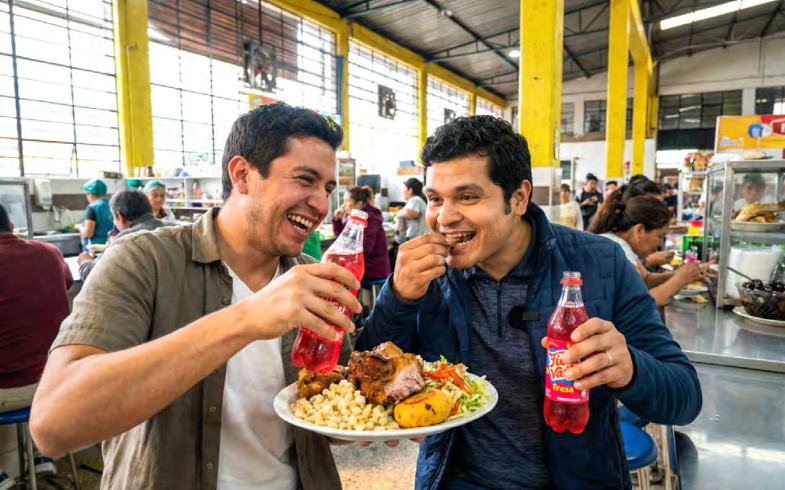
\includegraphics[width=\textwidth]{figs/fig_mercado.png}}\par
      \vspace{2pt}
      \tiny pag 70
      \end{center}
      \vspace{2pt}
      \begin{tcolorbox}[colback=arcaGray, colframe=codeGreen, leftrule=2pt,
        boxrule=0pt, sharp corners, left=4pt, right=4pt, top=2pt, bottom=2pt]
        {\tiny\color{textDark}\itshape
        ``Dos hombres disfrutando comida en un mercado. Se ven las marcas
        Inca Kola y Coca-Cola.''}
      \end{tcolorbox}
    \end{column}
    \begin{column}{0.32\textwidth}
      \begin{center}
      \fbox{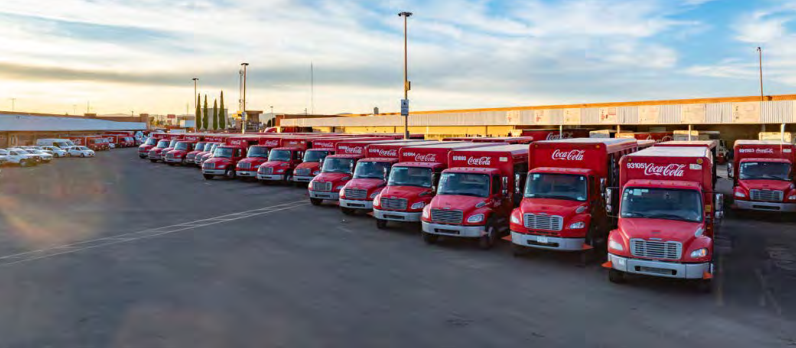
\includegraphics[width=\textwidth]{figs/fig_camiones.png}}\par
      \vspace{2pt}
      \tiny pag 47
      \end{center}
      \vspace{2pt}
      \begin{tcolorbox}[colback=arcaGray, colframe=codeGreen, leftrule=2pt,
        boxrule=0pt, sharp corners, left=4pt, right=4pt, top=2pt, bottom=2pt]
        {\tiny\color{textDark}\itshape
        ``Fila de camiones de Coca-Cola en un almacén, listos para
        la distribución de productos.''}
      \end{tcolorbox}
    \end{column}
    \begin{column}{0.32\textwidth}
      \begin{center}
      \fbox{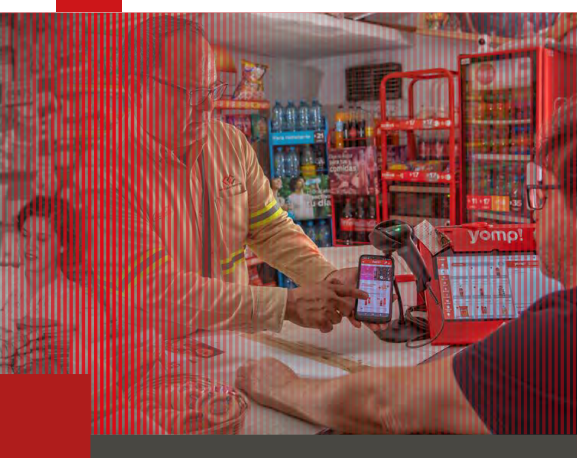
\includegraphics[width=\textwidth]{figs/fig_pago_movil.png}}\par
      \vspace{2pt}
      \tiny pag 61
      \end{center}
      \vspace{2pt}
      \begin{tcolorbox}[colback=arcaGray, colframe=codeGreen, leftrule=2pt,
        boxrule=0pt, sharp corners, left=4pt, right=4pt, top=2pt, bottom=2pt]
        {\tiny\color{textDark}\itshape
        ``Persona realizando pago móvil en una tienda de conveniencia, con
        refrigerador marca yomp!''}
      \end{tcolorbox}
    \end{column}
  \end{columns}
  \vspace{8pt}
  \begin{tcolorbox}[colback=arcaRed!8, colframe=arcaRed, leftrule=3pt,
    boxrule=0pt, sharp corners, left=8pt, right=8pt, top=4pt, bottom=4pt]
    {\footnotesize\color{arcaDark}\bfseries
    Scout identificó \emph{marcas, escenas, tecnología y contexto comercial}. Tres llamadas, tres textos listos para indexar.}
  \end{tcolorbox}
\end{frame}

% F31 — Cierre B4
\begin{frame}[shrink]{\faIndustry\ ¿Qué me llevo? --- Bloque 4}
  \vspace{6pt}
  \begin{itemize}\setlength{\itemsep}{5pt}
    \footnotesize
    \item \textbf{Captioning} convierte cualquier imagen en \emph{texto descriptivo}.
    \item El texto entra al RAG \emph{como si fuera otro chunk del manual}.
    \item Costo: \textbf{una llamada al VLM por imagen al indexar}. Cero costo extra en query.
  \end{itemize}
  \vspace{12pt}
  \begin{tcolorbox}[colback=arcaRed!8, colframe=arcaRed, leftrule=3pt,
    boxrule=0pt, sharp corners, left=8pt, right=8pt, top=4pt, bottom=4pt]
    {\footnotesize\color{arcaDark}\bfseries
    \emph{Captioning convierte la imagen en texto. Y ahí tu RAG ya funciona.}
    \faArrowRight\;Bloque 5: ahora, ¿hay alguna librería que ya haga \emph{todo
    esto} por nosotros?}
  \end{tcolorbox}
\end{frame}

% =============================================================================
%  BLOQUE 5 — pymupdf4llm: la librería que ya hace todo
% =============================================================================
\sectionframe{Bloque 5}{La librería que ya hace todo:\\\texttt{pymupdf4llm}}

% F33 — ¿Qué es pymupdf4llm?
\begin{frame}[shrink]{\texttt{pymupdf4llm}: parser de PDFs pensado para RAG}
  \vspace{8pt}
  \begin{tcolorbox}[colback=arcaGray, colframe=arcaRed, leftrule=3pt,
    boxrule=0pt, sharp corners, left=10pt, right=10pt, top=6pt, bottom=6pt]
    {\footnotesize\color{arcaDark}
    Una librería Python que toma tu PDF y te devuelve \textbf{markdown limpio},
    \textbf{detecta tablas} como markdown tabular, y \textbf{guarda las
    figuras como PNG} con un nombre que las ata a su página.}
  \end{tcolorbox}
  \vspace{10pt}
  \begin{itemize}\setlength{\itemsep}{4pt}
    \footnotesize
    \item Python puro, \texttt{pip install pymupdf4llm}. Sin servidor, sin API key.
    \item Reusa \texttt{pymupdf} (el mismo que mostramos antes).
    \item Licencia AGPL (open source).
    \item \textbf{Velocidad real medida:} 31 páginas del reporte Arca $\to$ \textbf{6.8 s}
    en una laptop. Sale 67 KB de markdown $+$ 108 PNGs.
  \end{itemize}
\end{frame}

% F34 — Qué hace
\begin{frame}[fragile, shrink]{Qué hace --- una sola línea}
  \begin{pyblock}
import pymupdf4llm

md = pymupdf4llm.to_markdown(
    "reporte_arca_2025.pdf",
    write_images=True,                  # guarda las figuras
    image_path="figs/",
    image_format="png",
)
print(len(md), "chars de markdown")    # 66612
print(os.listdir("figs/")[:3])          # ['...pdf-0001-03.png', ...]
  \end{pyblock}
  \vspace{6pt}
  \begin{tcolorbox}[colback=arcaRed!8, colframe=arcaRed, leftrule=3pt,
    boxrule=0pt, sharp corners, left=8pt, right=8pt, top=3pt, bottom=3pt]
    {\footnotesize\color{arcaDark}\bfseries
    Una llamada. Te devuelve el texto en \emph{markdown} (con encabezados,
    bullets, negritas detectadas) y te extrae \emph{cada imagen del PDF como un
    PNG aparte}.}
  \end{tcolorbox}
\end{frame}

% F35 — Output real sobre el reporte
\begin{frame}[shrink]{Lo que \texttt{pymupdf4llm} saca de esa misma página 44}
  \vspace{2pt}
  \begin{tcolorbox}[colback=arcaGray, colframe=codeGreen, leftrule=3pt,
    boxrule=0pt, sharp corners, left=8pt, right=8pt, top=4pt, bottom=4pt,
    title={\scriptsize\color{white}\bfseries\ttfamily pymupdf4llm.to\textunderscore markdown(...)},
    coltitle=white, colbacktitle=codeGreen, fonttitle=\scriptsize]
    {\scriptsize\color{textDark}\ttfamily
    MENSAJE PRÓLOGO~~~~ESTO ES AC~~~~NEGOCIO SOSTENIBLE~~~~CLIENTES\par
    \vspace{2pt}
    **44**\par
    \vspace{2pt}
    **==> picture [612 x 761] intentionally omitted <==**\par
    \vspace{2pt}
    \textbf{Comité de Sostenibilidad}\par
    Evolución de Modelo de Negocio Sostenible\par
    \vspace{2pt}
    Hoy, la sostenibilidad es un criterio que define inversiones,\par
    decisiones y relaciones con los grupos de interés, validado\par
    por estándares globales que reconocen la gestión responsable\par
    y la creación de valor a largo plazo.\par
    \vspace{2pt}
    Arca Continental forma parte de índices como el FTSE4Good de la\par
    Bolsa de Valores de Londres, que evalúa prácticas ambientales\par
    y sociales; Dow Jones Best-in-Class World Index\ldots\par}
  \end{tcolorbox}
  \vspace{4pt}
  \begin{tcolorbox}[colback=arcaRed!8, colframe=arcaRed, leftrule=3pt,
    boxrule=0pt, sharp corners, left=8pt, right=8pt, top=3pt, bottom=3pt]
    {\footnotesize\color{arcaDark}\bfseries
    Las palabras llegan enteras, los encabezados marcados con \texttt{**...**}.
    Los lugares donde había figura quedan marcados con \texttt{<== picture ==>}
    --- la imagen está en disco con su \emph{filename}.}
  \end{tcolorbox}
\end{frame}

% F36 — Diff PyPDF vs pymupdf4llm
\begin{frame}[shrink]{El diff de la página 44 --- PyPDF vs pymupdf4llm}
  \vspace{2pt}
  \begin{columns}[t]
    \begin{column}{0.49\textwidth}
      \begin{tcolorbox}[colback=arcaGray, colframe=arcaRed, leftrule=3pt,
        boxrule=0pt, sharp corners, left=6pt, right=6pt, top=4pt, bottom=4pt,
        title={\scriptsize\color{white}\bfseries\ttfamily PyPDF},
        coltitle=white, colbacktitle=arcaRed, fonttitle=\scriptsize]
        {\scriptsize\color{textDark}\ttfamily
        Comité \\ de \\ Sostenibilidad\par
        Evolución \\ de \\ Modelo \\ de\par
        S \\ ostenible\par
        Dow Jones Best \\ \textperiodcentered \\ in \\ \textperiodcentered \\ Class\par
        \vspace{4pt}
        {\color{arcaRed}\bfseries [\,figuras: ninguna\,]}}
      \end{tcolorbox}
    \end{column}
    \begin{column}{0.49\textwidth}
      \begin{tcolorbox}[colback=arcaGray, colframe=codeGreen, leftrule=3pt,
        boxrule=0pt, sharp corners, left=6pt, right=6pt, top=4pt, bottom=4pt,
        title={\scriptsize\color{white}\bfseries\ttfamily pymupdf4llm},
        coltitle=white, colbacktitle=codeGreen, fonttitle=\scriptsize]
        {\scriptsize\color{textDark}\ttfamily
        \textbf{Comité de Sostenibilidad}\par
        Evolución de Modelo de Negocio Sostenible\par
        Dow Jones Best-in-Class World Index\ldots\par
        \vspace{4pt}
        {\color{codeGreen}\bfseries [\,figuras extraídas en figs/:\par
        \,pdf-0004-02.png\par
        \,pdf-0004-03.png\par
        \,pdf-0004-05.png\,]}}
      \end{tcolorbox}
    \end{column}
  \end{columns}
  \vspace{10pt}
  \begin{tcolorbox}[colback=arcaRed!8, colframe=arcaRed, leftrule=3pt,
    boxrule=0pt, sharp corners, left=8pt, right=8pt, top=3pt, bottom=3pt]
    {\footnotesize\color{arcaDark}\bfseries
    \faCheckSquare~Texto limpio + figuras en archivos.
    Lo que falta: \emph{describir las figuras}. Eso es captioning.}
  \end{tcolorbox}
\end{frame}

% F37 — Pipeline completo
\begin{frame}[shrink]{El pipeline completo --- \texttt{pymupdf4llm} $+$ captioning}
  \vspace{6pt}
  \begin{center}
  \begin{tikzpicture}[font=\footnotesize, node distance=0.4cm and 0.5cm]
    \node[boxA, minimum width=2.0cm] (pdf) {\faFilePdf\\PDF};
    \node[boxBlue, right=of pdf, minimum width=2.2cm] (mu) {pymupdf4llm};
    \node[boxA, right=of mu, minimum width=2.0cm, align=center] (md) {markdown};
    \node[fill=codePurple, text=white, rounded corners=4pt, below=0.6cm of md,
          minimum width=2.0cm, minimum height=1cm, align=center,
          font=\bfseries\footnotesize] (figs) {\faImage\\figuras\\PNG};
    \draw[arrowR] (pdf) -- (mu); \draw[arrowR] (mu) -- (md);
    \draw[arrowR] (mu.south) -- ++(0,-0.4) -| (figs.north);

    \node[fill=arcaDark, text=white, rounded corners=4pt,
          right=of figs, minimum width=2.0cm, minimum height=1cm, align=center,
          font=\bfseries\footnotesize] (sc) {Scout\\caption};
    \node[boxA, right=of sc, minimum width=2.0cm] (cap) {captions\\texto};
    \draw[arrowR] (figs) -- (sc); \draw[arrowR] (sc) -- (cap);

    \node[boxGreen, right=of md, minimum width=2.0cm] (chunk) {chunks};
    \draw[arrowR] (md) -- (chunk);
    \draw[arrowR] (cap) -| (chunk);

    \node[boxBlue, below=0.6cm of chunk, minimum width=2.4cm] (store) {Chroma\\$+$ metadata};
    \draw[arrowR] (chunk) -- (store);
  \end{tikzpicture}
  \end{center}
  \vspace{10pt}
  \begin{tcolorbox}[colback=arcaRed!8, colframe=arcaRed, leftrule=3pt,
    boxrule=0pt, sharp corners, left=8pt, right=8pt, top=3pt, bottom=3pt]
    {\footnotesize\color{arcaDark}\bfseries
    Texto + figuras descritas, todo \emph{como texto}, todo en el mismo store,
    cada chunk con \texttt{metadata=\{...,\,modalidad\,:\,texto$|$figura\}}.}
  \end{tcolorbox}
\end{frame}

% F38 — Mapa de alternativas
\begin{frame}[shrink]{Si \texttt{pymupdf4llm} te queda chico --- el mapa}
  \vspace{6pt}
  \begin{center}
  \begin{tabular}{p{2.6cm} p{4.6cm} p{4.6cm}}
    \toprule
    \scriptsize\textbf{Herramienta} & \scriptsize\textbf{Qué agrega} & \scriptsize\textbf{Costo / fricción}\\
    \midrule
    \scriptsize\textbf{pymupdf4llm} & \scriptsize markdown limpio, figuras a PNG & \scriptsize free, Python, 7 s / 31 pp \\
    \scriptsize\textbf{Docling} (IBM) & \scriptsize layout, OCR, tablas estructuradas & \scriptsize free, pesado: \texttt{$\sim$8 min / pág} en este PDF \\
    \scriptsize\textbf{LlamaParse} & \scriptsize layout vía LLM, tablas excelentes & \scriptsize API paga (free tier limitado) \\
    \scriptsize\textbf{Unstructured} & \scriptsize ingesta de muchos formatos, layout & \scriptsize free, dependencias pesadas \\
    \scriptsize\textbf{RAGFlow} (app) & \scriptsize \emph{pipeline completo con UI web} & \scriptsize Docker, multiusuario \\
    \bottomrule
  \end{tabular}
  \end{center}
  \vspace{10pt}
  \begin{tcolorbox}[colback=arcaGray, colframe=arcaRed, leftrule=3pt,
    boxrule=0pt, sharp corners, left=8pt, right=8pt, top=4pt, bottom=4pt]
    {\footnotesize\color{arcaDark}
    Default Arca: \textbf{pymupdf4llm}. Si el PDF tiene \emph{tablas
    críticas para el negocio} y los números no pueden salir mal: LlamaParse o
    Docling. Si quieres algo \emph{con UI para que los usuarios suban sus
    propios PDFs}: RAGFlow.}
  \end{tcolorbox}
\end{frame}

% F39 — Cierre B5
\begin{frame}[shrink]{\faIndustry\ ¿Qué me llevo? --- Bloque 5}
  \vspace{6pt}
  \begin{itemize}\setlength{\itemsep}{5pt}
    \footnotesize
    \item Probablemente \textbf{no quieres escribir tu propio parser}. Hay
    librerías que ya hacen el 90\,\%.
    \item Para arrancar: \textbf{pymupdf4llm}. Una línea. Te da markdown $+$
    figuras.
    \item Cuando el negocio depende de \textbf{precisión sobre tablas} o tienes
    \textbf{PDFs escaneados}, subes a Docling / LlamaParse.
  \end{itemize}
  \vspace{12pt}
  \begin{tcolorbox}[colback=arcaRed!8, colframe=arcaRed, leftrule=3pt,
    boxrule=0pt, sharp corners, left=8pt, right=8pt, top=4pt, bottom=4pt]
    {\footnotesize\color{arcaDark}\bfseries
    \emph{Esto ya existe como librería. Docling te lo resuelve.}
    \faArrowRight\;Bloque 6: armemos el asistente Arca v2.}
  \end{tcolorbox}
\end{frame}

% =============================================================================
%  BLOQUE 6 — Asistente Arca v2
% =============================================================================
\sectionframe{Bloque 6}{El asistente Arca v2\\sobre el Reporte 2025}

% F41 — Arquitectura final
\begin{frame}[shrink]{Arquitectura del asistente v2}
  \vspace{4pt}
  \begin{center}
  \begin{tikzpicture}[font=\footnotesize, node distance=0.35cm and 0.45cm]
    %% Ingesta texto
    \node[boxA, minimum width=2.0cm] (pdf) {\faFilePdf\\reporte};
    \node[boxBlue, right=of pdf, minimum width=2.2cm] (mu) {pymupdf4llm};
    \node[boxA, right=of mu, minimum width=2.0cm] (md) {markdown};
    \node[boxA, right=of md, minimum width=1.6cm] (txt) {chunks\\texto};
    \draw[arrowR] (pdf) -- (mu); \draw[arrowR] (mu) -- (md); \draw[arrowR] (md) -- (txt);

    %% Ingesta figuras
    \node[fill=codePurple, text=white, rounded corners=4pt, below=0.4cm of md,
          minimum width=2.0cm, minimum height=0.9cm, align=center,
          font=\bfseries\footnotesize] (figs) {figs PNG};
    \node[fill=arcaDark, text=white, rounded corners=4pt, right=of figs,
          minimum width=2.0cm, minimum height=0.9cm, align=center,
          font=\bfseries\footnotesize] (cap) {Scout\\caption};
    \draw[arrowR] (mu.south) to[bend right=0] (figs.north);
    \draw[arrowR] (figs) -- (cap);

    %% Embedding compartido
    \node[boxGreen, right=of cap, minimum width=2.0cm] (emb) {embed\\mpnet};
    \draw[arrowR] (cap) -- (emb);
    \draw[arrowR] (txt.south) |- (emb.north);

    %% Chroma
    \node[boxBlue, below=0.4cm of emb, minimum width=2.6cm, align=center]
         (db) {Chroma\\\tiny metadata: modalidad};
    \draw[arrowR] (emb) -- (db);

    %% Query
    \node[boxA, left=2.2cm of db, minimum width=2.0cm, align=center]
         (q) {pregunta\\del usuario};
    \node[fill=arcaDark, text=white, rounded corners=4pt, below=0.4cm of db,
          minimum width=2.0cm, minimum height=0.9cm, align=center,
          font=\bfseries\footnotesize] (llm) {LLM};
    \node[boxGreen, left=of llm, minimum width=2.0cm] (ans) {respuesta\\+ cita};
    \draw[arrowR] (q) -- (db);
    \draw[arrowR] (db) -- (llm);
    \draw[arrowR] (llm) -- (ans);
  \end{tikzpicture}
  \end{center}
  \vspace{6pt}
  \begin{tcolorbox}[colback=arcaRed!8, colframe=arcaRed, leftrule=3pt,
    boxrule=0pt, sharp corners, left=8pt, right=8pt, top=3pt, bottom=3pt]
    {\footnotesize\color{arcaDark}\bfseries
    Texto $+$ captions van al mismo store. La metadata
    (\texttt{modalidad}) deja filtrar en el query.}
  \end{tcolorbox}
\end{frame}

% F42 — Pipeline en código
\begin{frame}[fragile, shrink]{Pipeline en código --- una pasada}
  \begin{pyblock}
md = pymupdf4llm.to_markdown("reporte.pdf",
                             write_images=True, image_path="figs/")
chunks_txt = sliding_window(md, tam=400)
chunks_img = [caption(p) for p in glob("figs/*.png")]

docs   = chunks_txt + chunks_img
metas  = [{"modalidad":"texto"}]*len(chunks_txt) + \
         [{"modalidad":"figura"}]*len(chunks_img)

embs = embedder.encode(docs, normalize_embeddings=True).tolist()
col.add(documents=docs, embeddings=embs, metadatas=metas,
        ids=[f"d_{i}" for i in range(len(docs))])
  \end{pyblock}
  \vspace{4pt}
  \begin{tcolorbox}[colback=arcaRed!8, colframe=arcaRed, leftrule=3pt,
    boxrule=0pt, sharp corners, left=8pt, right=8pt, top=3pt, bottom=3pt]
    {\footnotesize\color{arcaDark}\bfseries
    El \texttt{rag(pregunta)} de clase 35 \emph{no cambia ni una línea}.}
  \end{tcolorbox}
\end{frame}

% F43 — Demo query texto
\begin{frame}[shrink]{Query \#1 --- pregunta de texto sobre el reporte}
  \vspace{2pt}
  \begin{tcolorbox}[colback=arcaGray, colframe=codeBlue, leftrule=3pt,
    boxrule=0pt, sharp corners, left=8pt, right=8pt, top=4pt, bottom=4pt,
    title={\scriptsize\color{white}\bfseries Pregunta},
    coltitle=white, colbacktitle=codeBlue, fonttitle=\scriptsize]
    {\footnotesize\color{textDark}
    \itshape ``¿En qué índices de sostenibilidad está Arca Continental?''}
  \end{tcolorbox}
  \vspace{4pt}
  \begin{tcolorbox}[colback=arcaGray, colframe=codeOrange, leftrule=3pt,
    boxrule=0pt, sharp corners, left=8pt, right=8pt, top=4pt, bottom=4pt,
    title={\scriptsize\color{white}\bfseries Top-3 (mezcla texto $+$ caption)},
    coltitle=white, colbacktitle=codeOrange, fonttitle=\scriptsize]
    {\scriptsize\color{textDark}
    \textbf{[texto]} ``Arca Continental forma parte de índices como el FTSE4Good\ldots\
    Dow Jones Best-in-Class World Index\ldots\ Sustainability Yearbook de S\&P
    Global desde 2022\ldots''\par
    \textbf{[figura]} ``Página de reporte con logos: S\&P Global, Sustainalytics,
    Dow Jones, MSCI, FTSE4Good, CDP, GRI, Ellen MacArthur Foundation\ldots''}
  \end{tcolorbox}
  \vspace{4pt}
  \begin{tcolorbox}[colback=arcaGray, colframe=codeGreen, leftrule=3pt,
    boxrule=0pt, sharp corners, left=8pt, right=8pt, top=4pt, bottom=4pt,
    title={\scriptsize\color{white}\bfseries Respuesta del LLM},
    coltitle=white, colbacktitle=codeGreen, fonttitle=\scriptsize]
    {\scriptsize\color{textDark}
    Arca está en FTSE4Good (Londres), Dow Jones Best-in-Class World Index,
    Sustainability Yearbook de S\&P desde 2022. También figura en MSCI, CDP, GRI y
    Ellen MacArthur Foundation \emph{(visto en la página de logos)}.}
  \end{tcolorbox}
\end{frame}

% F44 — Demo query con imagen
\begin{frame}[shrink]{Query \#2 --- recuperación que llega \emph{vía una figura}}
  \vspace{2pt}
  \begin{tcolorbox}[colback=arcaGray, colframe=codeBlue, leftrule=3pt,
    boxrule=0pt, sharp corners, left=8pt, right=8pt, top=4pt, bottom=4pt,
    title={\scriptsize\color{white}\bfseries Pregunta},
    coltitle=white, colbacktitle=codeBlue, fonttitle=\scriptsize]
    {\footnotesize\color{textDark}
    \itshape ``¿Arca tiene presencia en mercados callejeros en Latinoamérica?''}
  \end{tcolorbox}
  \vspace{4pt}
  \begin{tcolorbox}[colback=arcaGray, colframe=codeOrange, leftrule=3pt,
    boxrule=0pt, sharp corners, left=8pt, right=8pt, top=4pt, bottom=4pt,
    title={\scriptsize\color{white}\bfseries Top-1 recuperado},
    coltitle=white, colbacktitle=codeOrange, fonttitle=\scriptsize]
    {\scriptsize\color{textDark}
    \textbf{[figura]} ``Dos hombres disfrutando comida en un mercado. Se ven las
    marcas Inca Kola y Coca-Cola.''}
  \end{tcolorbox}
  \vspace{4pt}
  \begin{tcolorbox}[colback=arcaRed!8, colframe=arcaRed, leftrule=3pt,
    boxrule=0pt, sharp corners, left=8pt, right=8pt, top=4pt, bottom=4pt]
    {\footnotesize\color{arcaDark}\bfseries
    Sin la \emph{descripción de la foto}, esa información \textbf{no estaba
    en el texto plano del PDF}. El captioning la rescató.}
  \end{tcolorbox}
\end{frame}

% F45 — Gradio
\begin{frame}[fragile, shrink]{Gradio --- lo muestras al supervisor el martes}
  \begin{pyblock}
import gradio as gr

def chat_arca(pregunta):
    return rag(pregunta, k=5)

gr.Interface(
    fn=chat_arca,
    inputs=gr.Textbox(label="Preguntá al Reporte Anual Arca 2025"),
    outputs=gr.Textbox(label="Respuesta + cita"),
    examples=["¿En qué índices ESG está Arca?",
              "¿Qué iniciativas tienen para reducir emisiones?",
              "¿Cuántos países opera Arca?"],
).launch(share=True)
  \end{pyblock}
  \vspace{4pt}
  \begin{tcolorbox}[colback=arcaRed!8, colframe=arcaRed, leftrule=3pt,
    boxrule=0pt, sharp corners, left=8pt, right=8pt, top=3pt, bottom=3pt]
    {\footnotesize\color{arcaDark}\bfseries
    URL pública de Colab. Sin despliegue. \emph{Funciona ya.}}
  \end{tcolorbox}
\end{frame}

% F46 — 3 ejercicios PBL
\begin{frame}[shrink]{Tres ejercicios para hoy}
  \vspace{6pt}
  \begin{tcolorbox}[colback=arcaGray, colframe=codeBlue, leftrule=3pt,
    boxrule=0pt, sharp corners, left=8pt, right=8pt, top=4pt, bottom=4pt,
    title={\scriptsize\color{white}\bfseries E1 --- aumentar la cobertura},
    coltitle=white, colbacktitle=codeBlue, fonttitle=\scriptsize]
    {\footnotesize\color{textDark}
    Re-indexa el reporte completo (189 pp). Compará 3 respuestas antes/después
    de agregar las 80 páginas de financieros.}
  \end{tcolorbox}
  \vspace{4pt}
  \begin{tcolorbox}[colback=arcaGray, colframe=codeOrange, leftrule=3pt,
    boxrule=0pt, sharp corners, left=8pt, right=8pt, top=4pt, bottom=4pt,
    title={\scriptsize\color{white}\bfseries E2 --- tu propio PDF},
    coltitle=white, colbacktitle=codeOrange, fonttitle=\scriptsize]
    {\footnotesize\color{textDark}
    Subí un PDF tuyo (otro reporte, manual, política), pásalo por pymupdf4llm,
    indexalo. Tres queries que muestren el valor.}
  \end{tcolorbox}
  \vspace{4pt}
  \begin{tcolorbox}[colback=arcaGray, colframe=codeGreen, leftrule=3pt,
    boxrule=0pt, sharp corners, left=8pt, right=8pt, top=4pt, bottom=4pt,
    title={\scriptsize\color{white}\bfseries E3 --- comparar dos librerías},
    coltitle=white, colbacktitle=codeGreen, fonttitle=\scriptsize]
    {\footnotesize\color{textDark}
    Ejecutá \texttt{pymupdf4llm} y luego (opcional) \texttt{docling} sobre el
    mismo PDF. Pegá los outputs lado a lado en una celda. ¿Cuál sirve para tu caso?}
  \end{tcolorbox}
\end{frame}

% F47 — Cierre B6
\begin{frame}[shrink]{\faIndustry\ ¿Qué me llevo? --- Bloque 6}
  \vspace{6pt}
  \begin{itemize}\setlength{\itemsep}{5pt}
    \footnotesize
    \item El \textbf{asistente Arca v2} responde sobre el reporte real, citando
    texto \emph{y} figuras.
    \item \textbf{La arquitectura no cambió respecto a clase 35.} Solo
    mejoramos la ingesta (pymupdf4llm $+$ captioning).
    \item Lo armas \emph{esta tarde} y lo muestras el lunes.
  \end{itemize}
  \vspace{12pt}
  \begin{tcolorbox}[colback=arcaRed!8, colframe=arcaRed, leftrule=3pt,
    boxrule=0pt, sharp corners, left=8pt, right=8pt, top=4pt, bottom=4pt]
    {\footnotesize\color{arcaDark}\bfseries
    \emph{Un asistente Arca v2 con todo junto. Lo armas hoy.}}
  \end{tcolorbox}
\end{frame}

% =============================================================================
%  BLOQUE 7 — Bonus: RAG sobre tablas para insights
% =============================================================================
\sectionframe{Bonus}{¿Y si el dato son números?\\RAG sobre tablas para insights}

% Bonus-1 — Por qué no le pasamos la tabla entera
\begin{frame}[shrink]{El dato son números, y la tabla es grande}
  \vspace{8pt}
  \begin{tcolorbox}[colback=arcaGray, colframe=arcaRed, leftrule=3pt,
    boxrule=0pt, sharp corners, left=8pt, right=8pt, top=6pt, bottom=6pt]
    {\footnotesize\color{arcaDark}
    Hasta aquí el RAG \emph{busca párrafos}. Pero a veces la pregunta es
    \emph{``de los 254 países del dataset OWID CO2, ¿cuáles fueron los 5 mayores
    emisores en 2022?''}.\par
    \vspace{4pt}
    Esa tabla tiene \textbf{50.411 filas $\times$ 79 columnas}.
    \textbf{No cabe en el contexto del LLM.} Y aunque cupiera,
    sería desperdicio: el LLM no es bueno para sumar miles de números.}
  \end{tcolorbox}
  \vspace{12pt}
  \begin{center}
  \begin{tikzpicture}[font=\footnotesize, node distance=0.5cm and 0.55cm]
    \node[boxA, align=center, minimum width=2.6cm] (q) {pregunta\\del usuario};
    \node[fill=arcaDark, text=white, rounded corners=4pt, right=of q,
          minimum width=2.0cm, minimum height=0.9cm, align=center,
          font=\bfseries\footnotesize] (l) {LLM};
    \node[fill=codeOrange, text=white, rounded corners=4pt, right=of l,
          minimum width=2.4cm, minimum height=0.9cm, align=center,
          font=\bfseries\footnotesize] (t) {tool call\\\texttt{df.groupby(\ldots)}};
    \node[boxBlue, right=of t, minimum width=1.8cm] (p) {pandas\\runtime};
    \node[boxGreen, below=0.6cm of p, minimum width=1.8cm] (r) {resultado};
    \draw[arrowR] (q) -- (l); \draw[arrowR] (l) -- (t); \draw[arrowR] (t) -- (p);
    \draw[arrowR] (p) -- (r);
    \draw[arrowR] (r) to[bend right=15] (l.south);
  \end{tikzpicture}
  \end{center}
  \vspace{6pt}
  \begin{tcolorbox}[colback=arcaRed!8, colframe=arcaRed, leftrule=3pt,
    boxrule=0pt, sharp corners, left=8pt, right=8pt, top=3pt, bottom=3pt]
    {\footnotesize\color{arcaDark}\bfseries
    Patrón: el LLM no \emph{mira} la tabla; el LLM \emph{pide al runtime}
    que la consulte por él. Eso es \emph{tool use}.}
  \end{tcolorbox}
\end{frame}

% Bonus-2 — El loop en código
\begin{frame}[fragile, shrink]{El loop completo (el agente lo ejecuta solo)}
  \begin{pyblock}
TOOLS = [{"type":"function", "function":{
    "name":"ejecutar_pandas",
    "description":"Ejecuta una expresion pandas sobre el DataFrame df.",
    "parameters":{"type":"object",
                  "properties":{"codigo":{"type":"string"}},
                  "required":["codigo"]}}}]

def agent(pregunta):
    msgs = [{"role":"system","content": SYSTEM},
            {"role":"user",  "content": pregunta}]
    for _ in range(4):
        r = client.chat.completions.create(model="llama-3.3-70b-versatile",
            messages=msgs, tools=TOOLS, tool_choice="auto")
        m = r.choices[0].message
        if not m.tool_calls: return m.content          # respuesta final
        msgs.append(m.model_dump())
        for tc in m.tool_calls:                         # ejecutar tool
            out = eval(json.loads(tc.function.arguments)["codigo"], {"df":df})
            msgs.append({"role":"tool","tool_call_id":tc.id,"content":str(out)})
  \end{pyblock}
  \vspace{2pt}
  {\footnotesize\color{arcaDark}
  El LLM \textbf{decide solo} cuándo llamar a la tool y cuándo terminar.
  \textbf{Tú escribes el loop una vez}; el modelo lo orquesta para cada pregunta.}
\end{frame}

% Bonus-3 — Demo real OWID CO2
\begin{frame}[shrink]{Demo real --- OWID CO2 (50.411 filas) preguntada en español}
  \vspace{2pt}
  \begin{tcolorbox}[colback=arcaGray, colframe=codeBlue, leftrule=3pt,
    boxrule=0pt, sharp corners, left=8pt, right=8pt, top=3pt, bottom=3pt,
    title={\scriptsize\color{white}\bfseries Pregunta},
    coltitle=white, colbacktitle=codeBlue, fonttitle=\scriptsize]
    {\footnotesize\color{textDark}
    \itshape ``¿Cuál es el CO2 per cápita de México vs Estados Unidos en 2022?''}
  \end{tcolorbox}
  \vspace{3pt}
  \begin{tcolorbox}[colback=arcaGray, colframe=codeOrange, leftrule=3pt,
    boxrule=0pt, sharp corners, left=8pt, right=8pt, top=3pt, bottom=3pt,
    title={\scriptsize\color{white}\bfseries Turn 1 --- el LLM genera la query},
    coltitle=white, colbacktitle=codeOrange, fonttitle=\scriptsize]
    {\scriptsize\color{textDark}\ttfamily
    df[(df['iso\textunderscore code'].notna()) \& (df['year']==2022) \&\par
    \quad(df['country'].isin(['Mexico','United States']))]\par
    \quad[['country','co2\textunderscore per\textunderscore capita']]}
  \end{tcolorbox}
  \vspace{3pt}
  \begin{tcolorbox}[colback=arcaGray, colframe=codePurple, leftrule=3pt,
    boxrule=0pt, sharp corners, left=8pt, right=8pt, top=3pt, bottom=3pt,
    title={\scriptsize\color{white}\bfseries Runtime ejecuta y devuelve},
    coltitle=white, colbacktitle=codePurple, fonttitle=\scriptsize]
    {\scriptsize\color{textDark}\ttfamily
    ~~~~~~~~~~country~~co2\textunderscore per\textunderscore capita\par
    29681~~~~~~Mexico~~~~~~~~~~~~3.528\par
    48005~~United States~~~~~~~14.802}
  \end{tcolorbox}
  \vspace{3pt}
  \begin{tcolorbox}[colback=arcaGray, colframe=codeGreen, leftrule=3pt,
    boxrule=0pt, sharp corners, left=8pt, right=8pt, top=3pt, bottom=3pt,
    title={\scriptsize\color{white}\bfseries Turn 2 --- el LLM redacta el insight},
    coltitle=white, colbacktitle=codeGreen, fonttitle=\scriptsize]
    {\scriptsize\color{textDark}\itshape
    ``El CO2 per cápita de México en 2022 fue de \textbf{3.528 toneladas},
    mientras que el de Estados Unidos fue de \textbf{14.802}. Esto muestra
    que Estados Unidos tiene una emisión per cápita \textbf{4.2 veces mayor}
    que la de México en 2022.''}
  \end{tcolorbox}
\end{frame}

% =============================================================================
%  CIERRE
% =============================================================================
\sectionframe{Cierre}{Lo que te llevas}

% F49 — Respuesta a la pregunta del día
\begin{frame}[shrink]{La respuesta a la pregunta del día}
  \vspace{4pt}
  \begin{tcolorbox}[colback=arcaDark, colframe=arcaDark, sharp corners,
    boxrule=0pt, left=10pt, right=10pt, top=5pt, bottom=5pt]
    {\footnotesize\color{white}\itshape
    En clase 35 armamos un chatbot Arca que cita el Código de Ética. Hoy queremos
    uno que lea el Reporte Anual Integrado 2025\ldots\ ¿por qué el RAG simple
    se rompe aquí, qué le ponemos para que funcione, y cuánto código real
    escribimos vs cuánto le pedimos a una librería profesional?\par}
  \end{tcolorbox}
  \vspace{10pt}
  \begin{tcolorbox}[colback=arcaRed!8, colframe=arcaRed, leftrule=3pt,
    boxrule=0pt, sharp corners, left=8pt, right=8pt, top=6pt, bottom=6pt]
    {\small\color{arcaDark}\bfseries
    \textbf{Se rompe} porque PyPDF aplana columnas, ignora figuras y destroza
    tablas.\par
    \vspace{2pt}
    \textbf{Lo arreglamos} con dos piezas: \emph{pymupdf4llm} (texto $+$
    extracción de figuras) y un \emph{modelo multimodal} (Scout) que describe
    cada figura.\par
    \vspace{2pt}
    \textbf{Escribimos $\sim$15 líneas propias}; el resto lo hace la librería.\par
    \vspace{4pt}
    \emph{Producción real $=$ librería pro $+$ multimodal $+$ RAG.}}
  \end{tcolorbox}
\end{frame}

% F50 — Gracias
\begin{frame}[plain, noframenumbering]
  \begin{tikzpicture}[remember picture, overlay]
    \fill[arcaDark] (current page.south west) rectangle (current page.north east);
    \node[anchor=center, text=white, font=\Huge\bfseries] at
      ([yshift=1cm]current page.center) {Gracias};
    \node[anchor=center, text=white!85, font=\Large] at
      ([yshift=-0.2cm]current page.center) {Preguntas?};
    \node[anchor=center, text=white!70, font=\small] at
      ([yshift=-1.5cm]current page.center)
      {Clase 36 --- RAG multimodal sobre el Reporte Arca 2025};
    \node[anchor=center, text=white!60, font=\scriptsize] at
      ([yshift=-2cm]current page.center)
      {github.com/cmosquerat/arca-diplomado/tree/main/clase-36};
  \end{tikzpicture}
\end{frame}

\end{document}
